\documentclass[10pt]{report}
\usepackage{amsmath}
\usepackage{graphicx}

\begin{document}
\title{CS663 Assignment-4 Question-1}
\author{KOTWAL ALANKAR SHASHIKANT}
\maketitle

\section*{Part A}
The output from the first part is shown below. The image on the left is the original image and the right image is the corrected image.

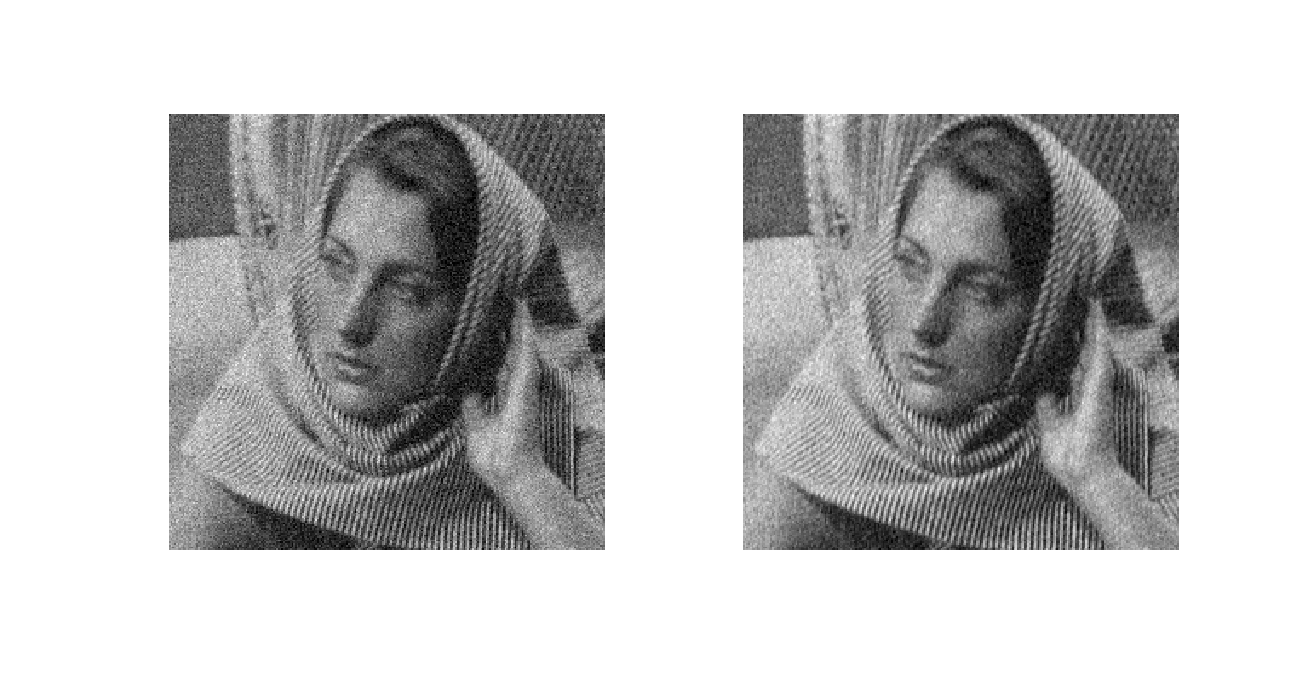
\includegraphics[scale=0.35]{out1}

The difference is more clear from the RMSDs. The RMSD for the corrupt image is 5121.6 while that for the corrected image is 3598.9. The noise image is shown below:

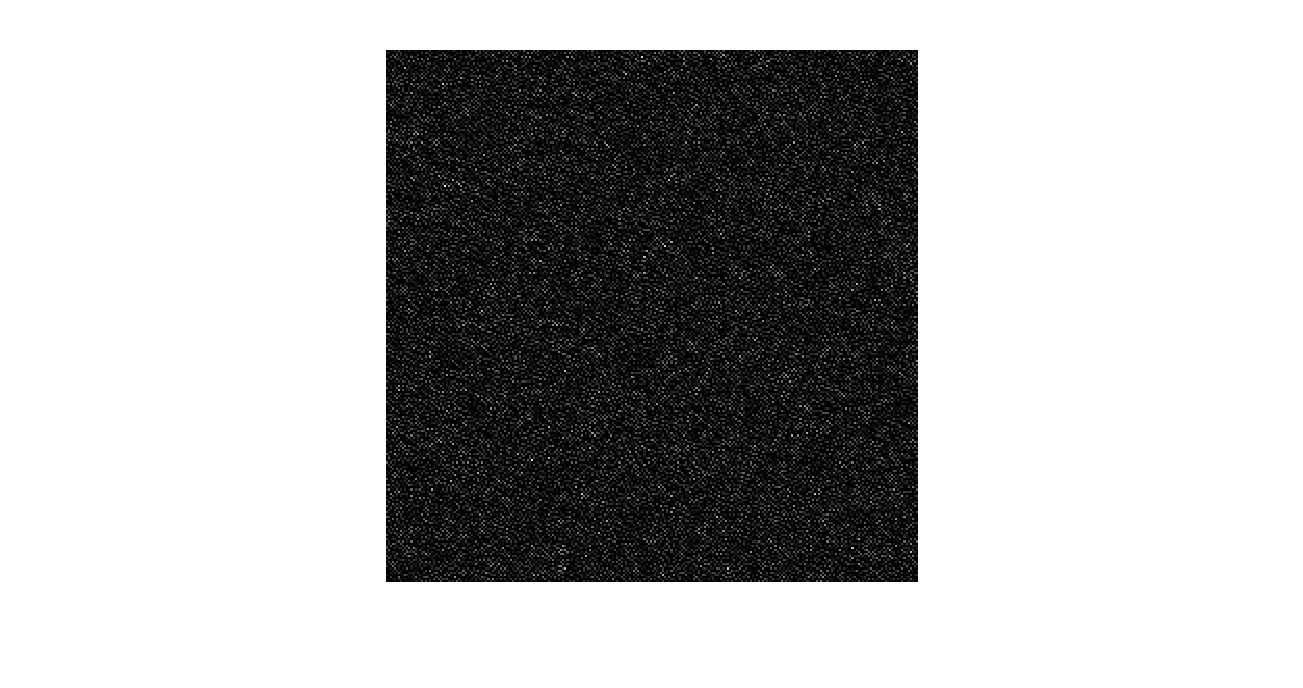
\includegraphics[scale=0.35]{noise1}

\newpage
\section*{Part B}
The denoising is more dramatic here. The output is shown below. The image on the left is the original image and the right image is the corrected image.

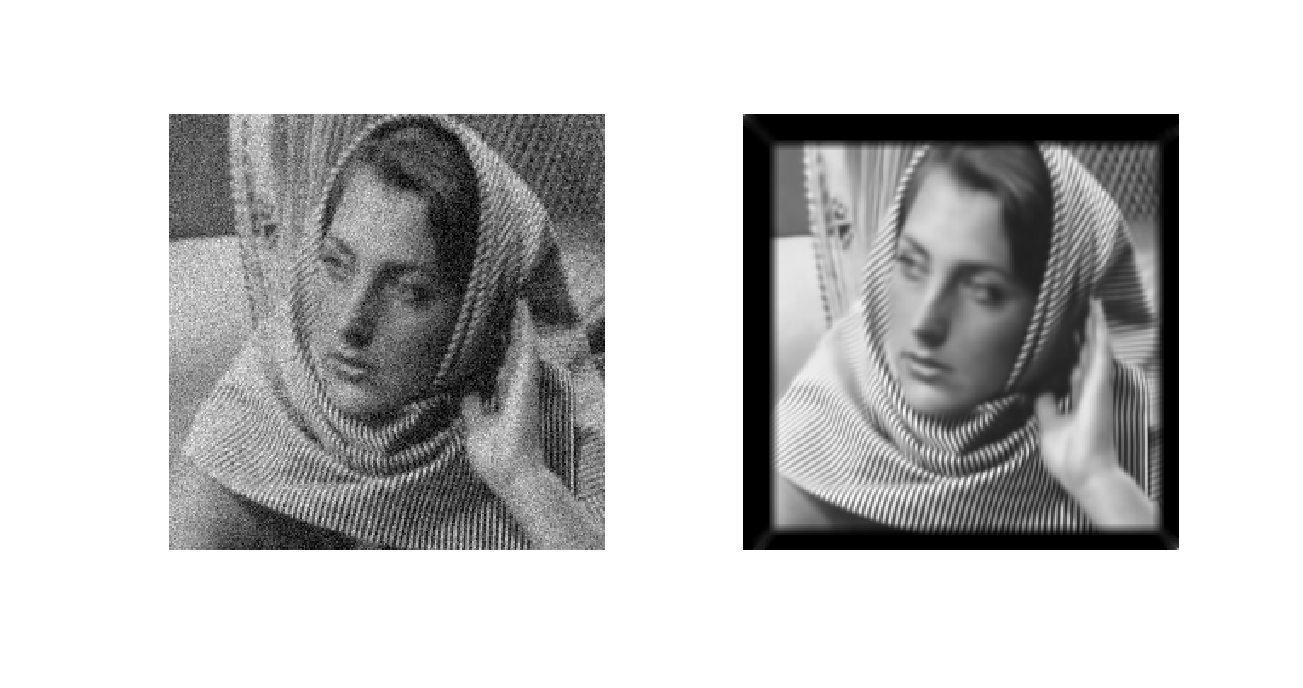
\includegraphics[scale=0.35]{out2}

There is a dark window on the image corners which is presumably caused by less patch data at the images edges.

\section*{Part C}
With the best parameters obtained for the bilateral filter for the image used at that time, the denoising is much less efficient. The output is shown below.

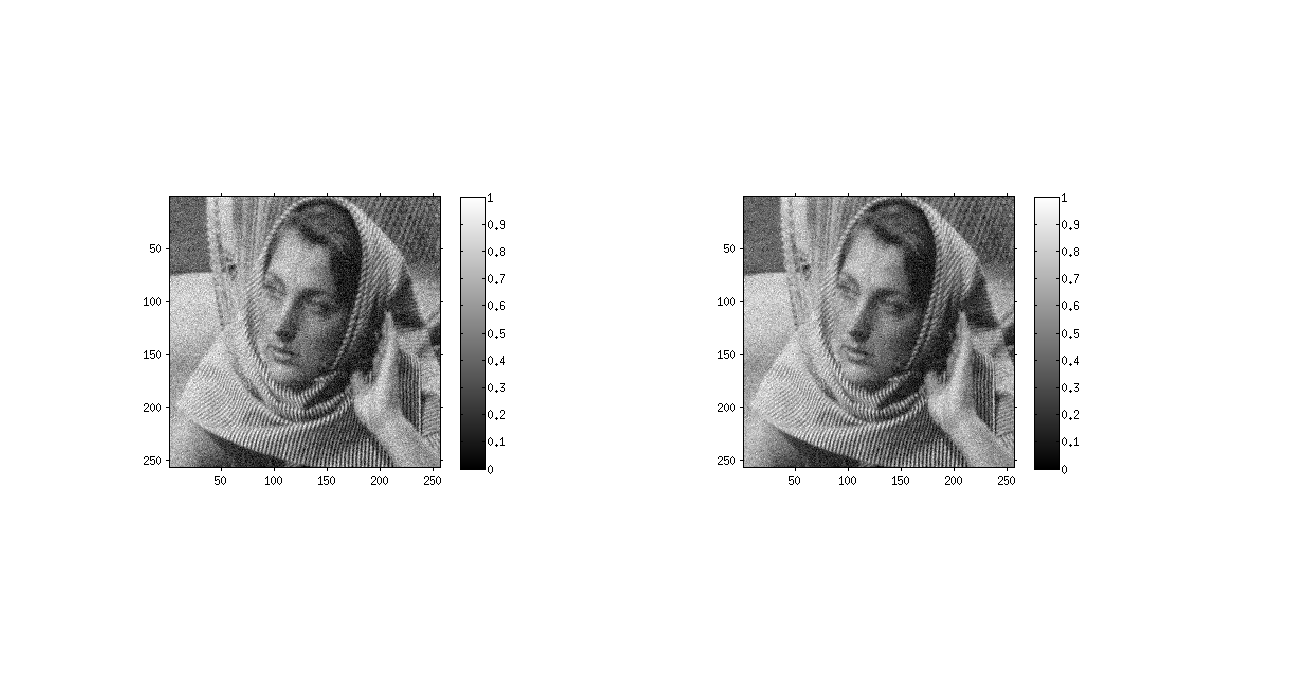
\includegraphics[scale=0.35]{out3}

(PTO)
\newpage
The main difference between the PCA-based technique and the bilateral filter is that the bilateral filter assigns weights based upon spatial and intensity difference only, while the PCA technique uses knowledge about the noise variance and estimates the denoised coefficients accordingly. So the PCA technique assumes an underlying noise model, while the bilateral filter tunes its parameters empirically.

\end{document}